\FloatBarrier
\section{Resultados}
\label{sec:results}

\subsection{Caracterização e conclusão da busca}

A Tabela~\ref{tab:characterization} caracteriza as
\TotalInstances{} instâncias do corpus, com intervalos calculados
dos arquivos efetivamente medidos. Os grafos aleatórios apresentam
de 2 a 313 arestas; as famílias estruturadas incluem tanto densidade
zero como densidade um. Esses extremos não representam a mesma
dificuldade para a busca, como mostram os resultados seguintes.

% Gerado dos CSVs reais por ReportStats.java.
\begin{table}[htbp]
\centering
\caption{Caracterização das 230 instâncias efetivamente medidas. Intervalos indicam mínimo e máximo observados por família; $d$ é a densidade.}
\label{tab:characterization}
\small
\begin{tabular}{lrrrr}
\toprule
Família & Quantidade & $n$ & $m$ & $d$ \\
\midrule
$G(n,p)$ & 200 & 10--30 & 2--313 & 0,038--0,778 \\
Caminho & 5 & 10--30 & 9--29 & 0,067--0,200 \\
Ciclo & 5 & 10--30 & 10--30 & 0,069--0,222 \\
Estrela & 5 & 10--30 & 9--29 & 0,067--0,200 \\
Completo & 5 & 10--30 & 45--435 & 1,000--1,000 \\
Bipartido completo & 5 & 10--30 & 25--225 & 0,517--0,556 \\
Sem arestas & 5 & 10--30 & 0--0 & 0,000--0,000 \\
\bottomrule
\end{tabular}
\end{table}


No resumo pelas medianas, o algoritmo exato retornou
\OptimalInstances{} resultados \texttt{OPTIMAL} e
\TimeoutInstances{} resultados \texttt{TIME\_LIMIT}.
Entre as \RawMeasurements{} medições individuais do exato,
\RawTimeouts{} atingiram o limite, três em cada uma das duas
instâncias não concluídas. A Figura~\ref{fig:status} apresenta
as contagens por instância, não por repetição.
As flags de validade do exato e da aproximação são verdadeiras
em todas as linhas dos dois CSVs, coerentemente com a validação
executada antes da exportação.

\begin{figure}[htbp]
\centering
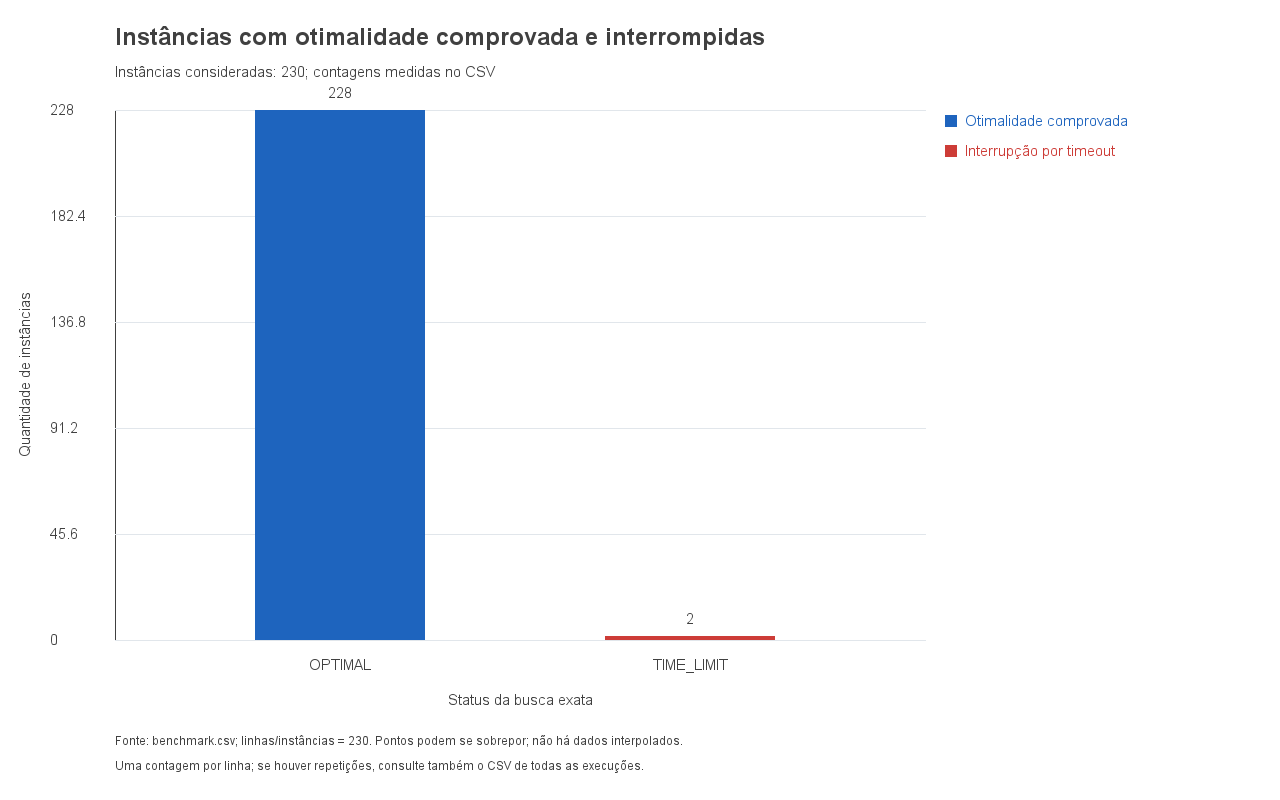
\includegraphics[width=\textwidth]{06-status.png}
\caption{Conclusão da busca exata nas 230 instâncias: 228 provas de ótimo e dois timeouts na execução selecionada de cada grafo. Fonte: benchmark original.}
\label{fig:status}
\end{figure}
\FloatBarrier

\subsection{Tempos por tamanho e densidade}

A Tabela~\ref{tab:configurations} apresenta as 20 configurações
aleatórias. A dispersão $[Q_1;Q_3]$ é calculada entre as dez
instâncias de cada par $(n,p)$, após a seleção das três medições
de cada algoritmo. As unidades diferentes são explícitas:
milissegundos para o exato e microssegundos para a aproximação.
O único timeout aleatório permanece como observação parcial.

% Gerado dos CSVs reais por ReportStats.java.
\begin{table}[htbp]
\centering
\caption{Tempos nos 200 grafos aleatórios: dez instâncias por configuração. Valores são medianas superiores entre instâncias, seguidas de $[Q_1;Q_3]$. A unidade do exato é ms e a da aproximação é $\mu$s. O tempo parcial do único timeout aleatório foi mantido; O/T conta ótimo/timeout.}
\label{tab:configurations}
\small
\setlength{\tabcolsep}{3pt}
\begin{tabular}{rrrrrl}
\toprule
$n$ & $p$ & $\bar d$ & Exato (ms) & Aprox. ($\mu$s) & O/T \\
\midrule
10 & 0,1 & 0,100 & 0,025 [0,022;0,028] & 5,70 [4,90;6,10] & 10/0 \\
10 & 0,3 & 0,289 & 0,039 [0,033;0,045] & 6,40 [5,80;6,60] & 10/0 \\
10 & 0,5 & 0,491 & 0,062 [0,047;0,097] & 3,20 [2,60;4,30] & 10/0 \\
10 & 0,7 & 0,729 & 0,067 [0,057;0,075] & 2,50 [2,20;2,80] & 10/0 \\
15 & 0,1 & 0,088 & 0,027 [0,015;0,036] & 1,40 [1,20;1,50] & 10/0 \\
15 & 0,3 & 0,276 & 0,102 [0,061;0,115] & 2,30 [2,00;2,60] & 10/0 \\
15 & 0,5 & 0,485 & 0,441 [0,258;0,485] & 3,30 [2,60;3,80] & 10/0 \\
15 & 0,7 & 0,677 & 1,251 [0,721;1,491] & 4,40 [2,90;5,20] & 10/0 \\
20 & 0,1 & 0,096 & 0,025 [0,017;0,028] & 1,70 [1,50;2,00] & 10/0 \\
20 & 0,3 & 0,289 & 0,482 [0,366;0,776] & 4,00 [3,50;4,50] & 10/0 \\
20 & 0,5 & 0,499 & 5,951 [2,461;6,214] & 5,10 [4,70;6,20] & 10/0 \\
20 & 0,7 & 0,702 & 6,152 [4,356;14,484] & 1,80 [1,50;2,00] & 10/0 \\
25 & 0,1 & 0,102 & 0,048 [0,033;0,053] & 0,70 [0,40;0,80] & 10/0 \\
25 & 0,3 & 0,293 & 1,992 [0,888;2,317] & 1,20 [1,10;1,70] & 10/0 \\
25 & 0,5 & 0,492 & 17,049 [13,597;19,951] & 1,90 [1,90;2,20] & 10/0 \\
25 & 0,7 & 0,710 & 133,245 [89,431;136,566] & 2,40 [2,10;2,40] & 10/0 \\
30 & 0,1 & 0,103 & 0,054 [0,036;0,157] & 0,70 [0,50;0,90] & 10/0 \\
30 & 0,3 & 0,295 & 22,094 [18,207;54,949] & 2,00 [1,90;2,10] & 10/0 \\
30 & 0,5 & 0,496 & 560,041 [218,852;586,354] & 2,30 [2,20;2,50] & 10/0 \\
30 & 0,7 & 0,685 & 3865,782 [2441,897;4069,889] & 2,60 [2,50;2,80] & 9/1 \\
\bottomrule
\end{tabular}
\end{table}


Para $p=0{,}5$, a mediana superior do exato entre instâncias
passa de 0,062~ms em $n=10$ para 560,041~ms em $n=30$.
Para $n=30$, varia de 0,054~ms em $p=0{,}1$ a
3\,865,782~ms em $p=0{,}7$, com um timeout na última configuração.
Na aproximação, as medianas das 20 configurações ficam entre
0,70 e 6,40~$\mu$s. Esses números são observações da execução,
e sua interpretação requer considerar a ordem da coleta e o
ambiente da JVM.

A Tabela~\ref{tab:sizes} agrega, para cada $n$, os 40 grafos
aleatórios das quatro probabilidades. A mediana de nós explorados
vai de 17 para 536\,777; a de podas, de 7 para 268\,385.
Cada coluna é agregada separadamente, e não representa
necessariamente uma mesma instância do grupo.

% Gerado dos CSVs reais por ReportStats.java.
\begin{table}[htbp]
\centering
\caption{Resumo por tamanho nos grafos aleatórios (40 instâncias por linha, quatro probabilidades). Tempos, nós e podas são medianas superiores entre instâncias. Contagens em timeout são parciais.}
\label{tab:sizes}
\small
\begin{tabular}{rrrrrr}
\toprule
$n$ & Exato (ms) & Aprox. ($\mu$s) & Nós & Podas & O/T \\
\midrule
10 & 0,050 & 4,90 & 17 & 7 & 40/0 \\
15 & 0,132 & 2,60 & 147 & 72 & 40/0 \\
20 & 1,276 & 3,50 & 1\,083 & 539 & 40/0 \\
25 & 7,451 & 1,90 & 27\,801 & 13\,897 & 40/0 \\
30 & 209,381 & 2,20 & 536\,777 & 268\,385 & 39/1 \\
\bottomrule
\end{tabular}
\end{table}


A Figura~\ref{fig:runtime} exibe os tempos das 230 instâncias,
incluindo as estruturadas. A escala logarítmica permite observar
as diferentes ordens de grandeza. As duas cruzes vermelhas são
tempos até interrupção, e não tempos completos para provar o
ótimo. Não há tempos nulos omitidos neste corpus.

\begin{figure}[htbp]
\centering
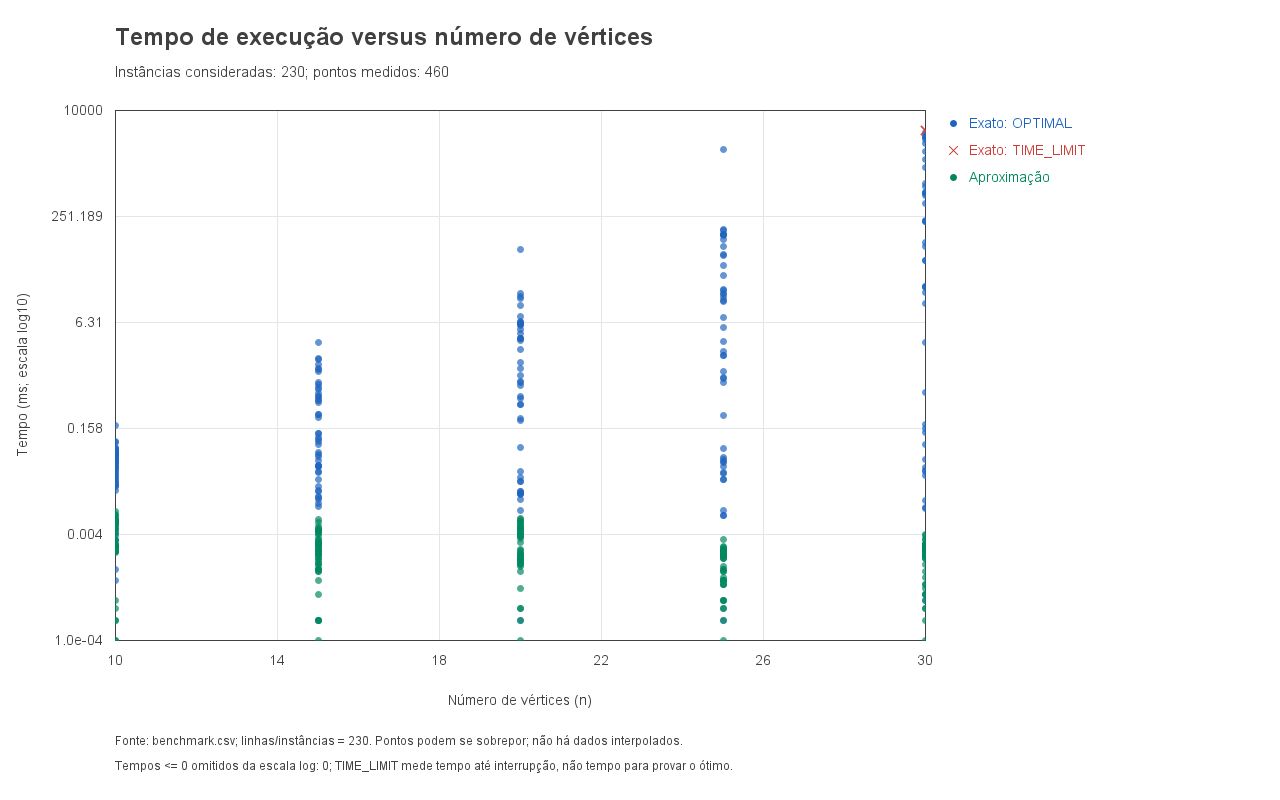
\includegraphics[width=\textwidth]{01-runtime-vs-n.png}
\caption{Tempo versus número de vértices nas 230 instâncias. São 460 pontos medidos, dois por grafo, sujeitos a sobreposição; o eixo vertical usa ms em escala logarítmica. Cruzes indicam timeout.}
\label{fig:runtime}
\end{figure}

A Figura~\ref{fig:density} utiliza a densidade observada da
Equação~\eqref{eq:density}, em vez de $p$. Ela reúne as sete
famílias; portanto, não isola o efeito da densidade do efeito
da estrutura ou de $n$. Para comparar configurações aleatórias
com tamanho fixado, deve-se consultar também a
Tabela~\ref{tab:configurations}.

\begin{figure}[htbp]
\centering
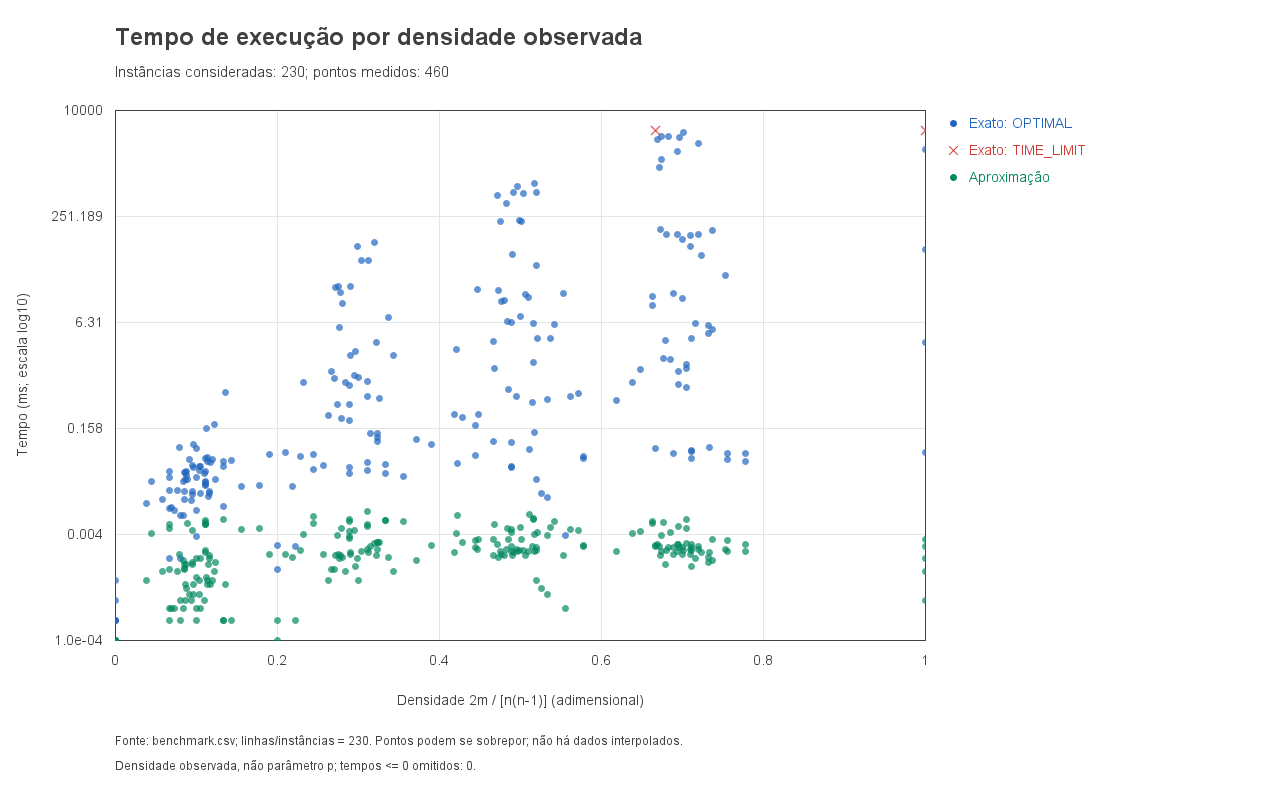
\includegraphics[width=\textwidth]{04-runtime-vs-density.png}
\caption{Tempos em ms por densidade observada: 230 instâncias e 460 pontos. O eixo vertical é logarítmico; valores em timeout são parciais. Famílias e tamanhos diferentes estão reunidos.}
\label{fig:density}
\end{figure}
\FloatBarrier

\subsection{Qualidade das coberturas}

A Tabela~\ref{tab:quality} apresenta as medidas da
Equação~\eqref{eq:quality}, incluindo somente as
\QualityInstances{} instâncias com ótimo comprovado e positivo.
A razão média é \MeanRatio{}, a mediana é \MedianRatio{} e o
gap médio é \MeanGap{}\%. Todas as razões elegíveis pertencem
ao intervalo $[1,2]$. Há \FactorTwoInstances{} casos com razão
exatamente dois. As \ZeroInstances{} instâncias com ótimo zero
retornam cobertura aproximada vazia e não participam dessas
estatísticas; os dois timeouts também são excluídos.

% Gerado dos CSVs reais por ReportStats.java.
\begin{table}[htbp]
\centering
\caption{Qualidade somente com ótimo comprovado e positivo. $\bar R$ é a média das razões individuais, não a razão de médias. Mediana e quartis referem-se a instâncias; gap médio em porcentagem.}
\label{tab:quality}
\small
\setlength{\tabcolsep}{4pt}
\begin{tabular}{lrrrrr}
\toprule
Amostra & $N$ & $\bar R$ & $R_{\mathrm{med}}$ $[Q_1;Q_3]$ & $R_{\max}$ & Gap médio (\%) \\
\midrule
Todas elegíveis & 223 & 1,493 & 1,400 [1,217;1,714] & 2,000 & 49,30 \\
Aleatórias & 199 & 1,453 & 1,385 [1,200;1,636] & 2,000 & 45,31 \\
Estruturadas & 24 & 1,823 & 2,000 [1,846;2,000] & 2,000 & 82,33 \\
\bottomrule
\end{tabular}
\end{table}


Nas instâncias com ótimo positivo, a aproximação coincide
em cardinalidade com o ótimo em \EqualPositiveInstances{} casos:
$K_{15}$ e $K_{25}$. Incluindo os cinco grafos sem arestas,
são \EqualTotalInstances{} coincidências. Isso não muda o
status do algoritmo aproximado para exato.

A Figura~\ref{fig:cover-size} contém as 228 instâncias com
ótimo comprovado, incluindo as cinco de ótimo zero.
As referências $y=x$ e $y=2x$ delimitam a igualdade com
o ótimo e a garantia teórica, respectivamente. A
Figura~\ref{fig:ratio} contém apenas as 223 razões definidas.
Pontos coincidentes não foram deslocados artificialmente.

\begin{figure}[htbp]
\centering
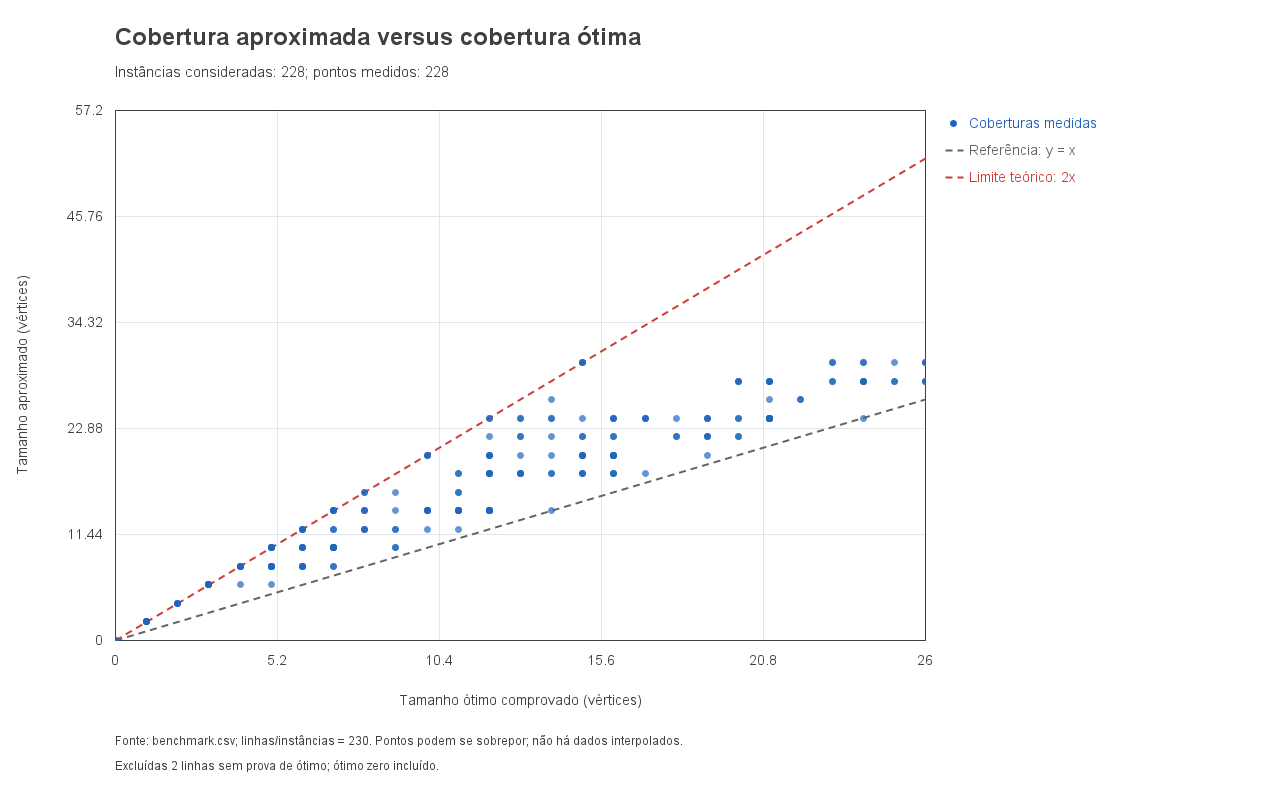
\includegraphics[width=\textwidth]{02-approx-vs-optimum.png}
\caption{Cardinalidade aproximada versus ótima em 228 instâncias com prova. Os dois timeouts são excluídos; ótimos zero são incluídos. Linhas tracejadas são referências teóricas, não medições.}
\label{fig:cover-size}
\end{figure}

\begin{figure}[htbp]
\centering
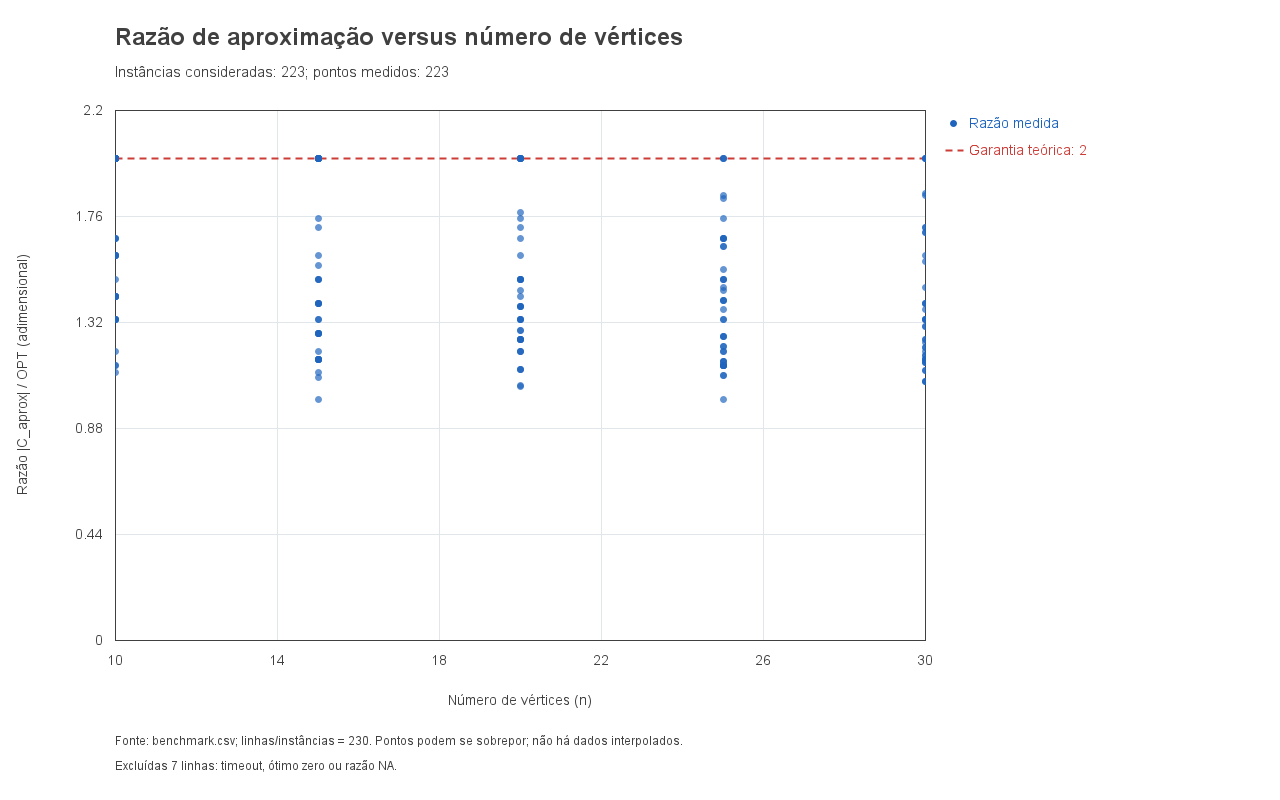
\includegraphics[width=\textwidth]{03-ratio-vs-n.png}
\caption{Razão de aproximação por número de vértices nas 223 instâncias elegíveis. Excluem-se dois timeouts e cinco ótimos zero. A linha em $R=2$ representa a garantia teórica.}
\label{fig:ratio}
\end{figure}
\FloatBarrier

\subsection{Famílias estruturadas e esforço de busca}

A Tabela~\ref{tab:structured} apresenta os 30 grafos estruturados.
O Branch and Bound comprova os valores de controle em 29 deles.
Somente $K_{30}$ termina em timeout. Nos caminhos, estrelas
e bipartidos completos deste conjunto, a aproximação utiliza
exatamente o dobro do ótimo. Os ciclos ímpares têm razões menores
que dois, e os completos ilustram coberturas aproximadas
próximas do mínimo, sem que isso torne simples a certificação
pela busca implementada.

% Gerado dos CSVs reais por ReportStats.java.
\begin{table}[htbp]
\centering
\caption{Resultados das 30 instâncias estruturadas (três medições por algoritmo; linha da mediana). Melhor é a incumbente exata; OPT é preenchido somente com prova. Tempos do exato em ms; nós são estados explorados.}
\label{tab:structured}
\small
\setlength{\tabcolsep}{4pt}
\begin{tabular}{lrrrrrr}
\toprule
Família & $n$ & Melhor & OPT & Aprox. & Exato (ms) & Nós \\
\midrule
Caminho & 10 & 5 & 5 & 10 & 0,0027 & 11 \\
Ciclo & 10 & 5 & 5 & 10 & 0,0026 & 11 \\
Estrela & 10 & 1 & 1 & 2 & 0,0012 & 3 \\
Completo & 10 & 9 & 9 & 10 & 0,0680 & 513 \\
Bipartido completo & 10 & 5 & 5 & 10 & 0,0039 & 11 \\
Sem arestas & 10 & 0 & 0 & 0 & 0,0008 & 0 \\
Caminho & 15 & 7 & 7 & 14 & 0,0425 & 15 \\
Ciclo & 15 & 8 & 8 & 14 & 0,0525 & 17 \\
Estrela & 15 & 1 & 1 & 2 & 0,0106 & 3 \\
Completo & 15 & 14 & 14 & 14 & 3,1101 & 16\,383 \\
Bipartido completo & 15 & 7 & 7 & 14 & 0,0144 & 15 \\
Sem arestas & 15 & 0 & 0 & 0 & 0,0002 & 0 \\
Caminho & 20 & 10 & 10 & 20 & 0,0093 & 21 \\
Ciclo & 20 & 10 & 10 & 20 & 0,0167 & 21 \\
Estrela & 20 & 1 & 1 & 2 & 0,0037 & 3 \\
Completo & 20 & 19 & 19 & 20 & 81,0001 & 524\,289 \\
Bipartido completo & 20 & 10 & 10 & 20 & 0,0168 & 21 \\
Sem arestas & 20 & 0 & 0 & 0 & 0,0002 & 0 \\
Caminho & 25 & 12 & 12 & 24 & 0,0077 & 25 \\
Ciclo & 25 & 13 & 13 & 24 & 0,0078 & 27 \\
Estrela & 25 & 1 & 1 & 2 & 0,0017 & 3 \\
Completo & 25 & 24 & 24 & 24 & 2621,2069 & 16\,777\,215 \\
Bipartido completo & 25 & 12 & 12 & 24 & 0,0268 & 25 \\
Sem arestas & 25 & 0 & 0 & 0 & 0,0002 & 0 \\
Caminho & 30 & 15 & 15 & 30 & 0,0099 & 31 \\
Ciclo & 30 & 15 & 15 & 30 & 0,0100 & 31 \\
Estrela & 30 & 1 & 1 & 2 & 0,0017 & 3 \\
Completo & 30 & 29 & NA & 30 & 5000,0004$^{*}$ & 31\,109\,928 \\
Bipartido completo & 30 & 15 & 15 & 30 & 0,1362 & 31 \\
Sem arestas & 30 & 0 & 0 & 0 & 0,0004 & 0 \\
\bottomrule
\end{tabular}

\smallskip
{\footnotesize $^{*}$TIME\_LIMIT: tempo e nós parciais; sem certificado de ótimo.}
\end{table}


A Figura~\ref{fig:nodes} apresenta todos os grafos, com
$\text{nós}+1$ no eixo vertical logarítmico para representar
também o caso zero. Grafos sem arestas não exigem estados
de busca. Em $K_{20}$ e $K_{25}$, os estados explorados são
524\,289 e 16\,777\,215, respectivamente; a razão entre
essas contagens é próxima de 32 para cinco vértices adicionais.
Em contraste, o bipartido completo com 30 vértices é resolvido
com 31 estados. São diferenças de estrutura, não apenas de tamanho.

\begin{figure}[htbp]
\centering
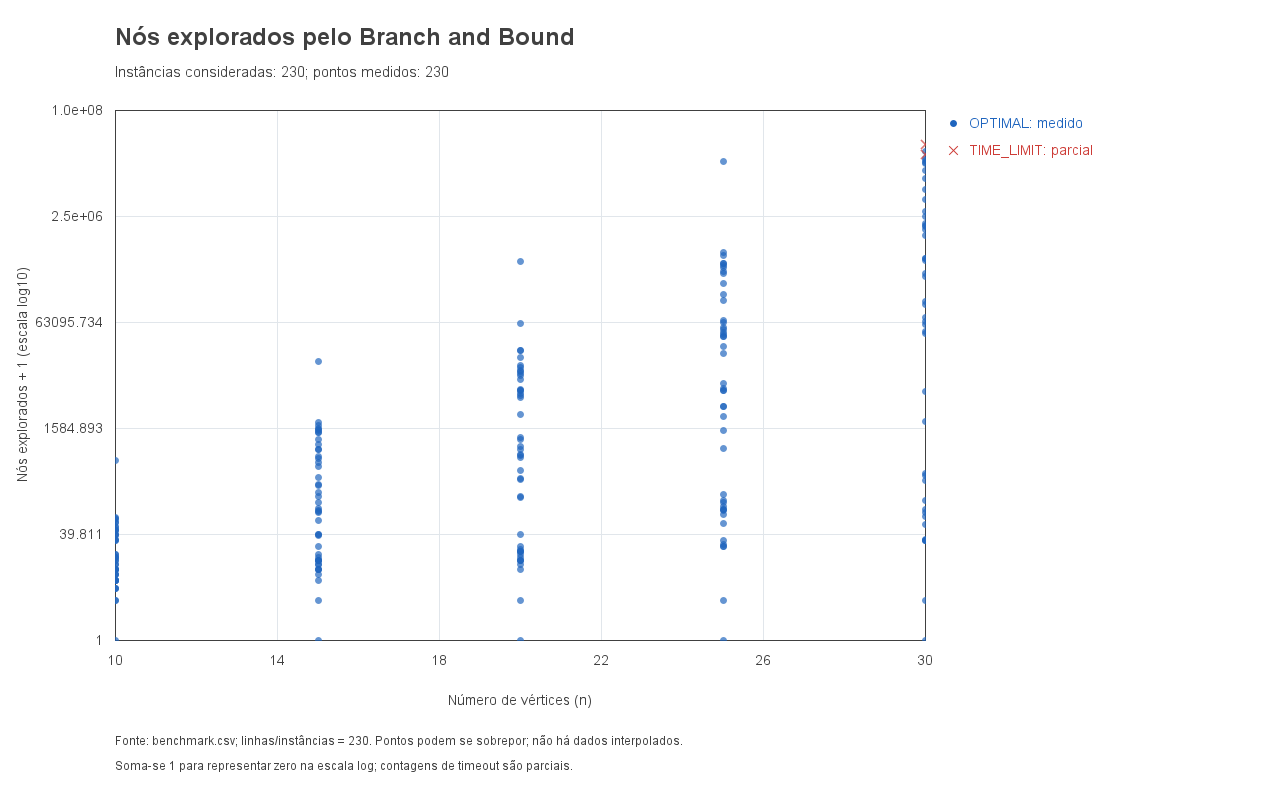
\includegraphics[width=\textwidth]{05-explored-nodes.png}
\caption{Estados explorados pelo Branch and Bound em 230 instâncias. O eixo vertical representa contagem mais um em escala logarítmica; cruzes vermelhas são contagens parciais de timeout.}
\label{fig:nodes}
\end{figure}
\FloatBarrier

\subsection{Instâncias interrompidas}

A Tabela~\ref{tab:timeouts} detalha os timeouts selecionados:
\path{random_n30_p0.7_i06}, com semente 20261311, e
\path{complete_n30}. As melhores coberturas conhecidas têm
tamanhos 26 e 29, enquanto a aproximação tem tamanhos 28 e 30.
Nenhuma razão ou gap é calculado a partir desses pares.

% Gerado dos CSVs reais por ReportStats.java.
\begin{table}[htbp]
\centering
\caption{As duas instâncias com TIME\_LIMIT no resumo. Tempos em ms e contagens pertencem às execuções selecionadas; ótimo, razão e gap são NA em ambas. Cada instância teve três timeouts nas medições individuais.}
\label{tab:timeouts}
\small
\setlength{\tabcolsep}{4pt}
\begin{tabular}{lrrrrr}
\toprule
Instância & Melhor & Aprox. & Tempo parcial & Nós & Podas \\
\midrule
$G(30;0{,}7)$, $i=6$ & 26 & 28 & 5000,0605 & 21\,986\,165 & 10\,993\,076 \\
$K_{30}$ & 29 & 30 & 5000,0004 & 31\,109\,928 & 15\,554\,955 \\
\bottomrule
\end{tabular}
\end{table}


As três medições de cada uma das duas instâncias foram
interrompidas, explicando os seis timeouts individuais.
O pequeno excesso em relação a 5\,000~ms é compatível com o
controle cooperativo do código. O registro global de
146,665~s inclui validação, exportação e progresso, não
sendo um tempo individual nem uma soma exclusiva das
chamadas dos algoritmos.
\FloatBarrier
